\chapter{本科毕业论文文献综述}
%字数要求3000字
%包括国内外现状、研究方向、进展情况、存在问题、参考依据

% 以game synchronization为中心(要不要加一个cheating avoidance?)
% (1)描述传统网络上同步算法如何 (参考已有文献综述)
% (2)描述ndn中同步算法发展到什么阶段
% (3)描述ndn的兄弟网络上同步算法发展到什么阶段(查找一下资料)

% 总的思路是说,首先同步是很重要的,其次同步的内容是很多的(包括结构和算法),再次NDN可以使P2P结构发挥很大优势,最后NDN目前对游戏的支持尚不多,尤其在同步这一块比较薄弱。说说其它的网络陪衬一番。
% 8月13日,若能在今天把这篇文章搞定,多好啊!

% 把CCN用于游戏中的好处:
% - 可以实现P2P架构,减短latency,增强robustness
% - 降低对带宽的要求,提升信息分享效率:每分数据至多走过一个链接一次,每个节点可以从离它最近的地方取到数据
%
% 不足:
% - P2P的安全问题尚未解决
% - P2P的同步机制比C/S复杂
% ————这是从游戏的角度说,游戏需要CCN,这个应该写在第一部分里面

% 从CCN的角度出发,CCN更需要游戏,因为没有任何一个网络不需要游戏的,因此综述里应该写各种不同的网络对游戏的支持(这样的话反倒应该看看那篇很宽泛的文章)——侧重于同步机制

\heiti
标题

\songti
不同网络中的多玩家网游同步机制

\heiti
摘要

\songti
最后写

\section{引言}
% 200字
% 任何一个网络设计师都不会忘记网络游戏,也不会忘记同步机制。
% 一句话介绍同步。
% 同步是很重要的
% 后续章节介绍
任何一个网络设计师都明白游戏对网络的重要性,也明白同步机制对于游戏的重要性。同步机制是保障游戏一致性(Consistency)的基本方法,而一致性是游戏得以公平、顺利开展的必要条件,是影响可玩度的一个重要因素。因此游戏所处的网络提供的服务和游戏所采用的同步机制常常可以影响一个游戏的命运。

在游戏产业发达的今天,网络游戏的开发者和设计者们已经积累了大量~IP~网络上的同步经验。然而随着新兴的数据命名网络的出现,游戏同步领域又产生了新的变化。

本文介绍了传统网络(以~IP~网络为代表)和新兴的数据命名网络(以~CCN~为代表)中的同步机制,综述了已有方法、发展状况和存在问题。~\ref{notion}~中介绍了网络游戏领域与同步相关的定义和标准,~\ref{traditional}~中介绍了传统~IP~网络中的经典同步机制,~\ref{innovative}~中介绍了新兴数据命名网络中的同步机制。


%============================%

\section{网络游戏与同步}
\label{notion}
% 同步的概念,
% 目标,是保持一致性 consistency
% 而 consistency,safety 的定义是有的
% 分类,分为asset, state吗?
% 同步与consistency, responsiveness有什么关系?
本节介绍了网络游戏的基本架构(\ref{archi}),游戏架构须提供的基本服务(\ref{service})和一致性的定义(\ref{def})。

\subsection{游戏架构}
% 400字
\label{archi}

多人在线游戏中的玩家是分散的,为此游戏设计者和网络工程师设计了不同的拓扑结构(或称游戏架构)来适应性地为分散的用户提供服务。这些拓扑结构可以分为三类:
\begin{itemize}
\item Client \/ Server Architecture~客户~\/~服务器架构
\item P2P Architecture~对等体架构
\item Distributed Architecture~分布式架构
\end{itemize}

\newcommand{\ioc}{I\/O\_C}

对这三种结构的具体描述见下文。这里需要概括的是:不论游戏采用哪种拓扑结构,它都由两类实体组成——输入输出控制实体(I\/O Client Control Entity,~简称~\ioc)和游戏状态服务器实体(Game State Server Entity,~简称~GSS)。\cite{Ferretti2005}

\ioc~通常是一个客户端软件,负责输入输出,对~GSS~收发事件(event)和图形渲染工作。~\ioc~可以看做游戏场景中一个或多个虚拟实体的拥有者,负责更新它们的属性(attribute)。\cite{hla}

\subsubsection{Client \/ Sserver~架构}
% 好处与缺点

客户~\/~服务器架构是商业界采用得最多的一种架构。~Quake \cite{quake}, Ultima Online \cite{ultima}~等游戏都采用此架构。


\begin{figure}[htbp]
\begin{center}
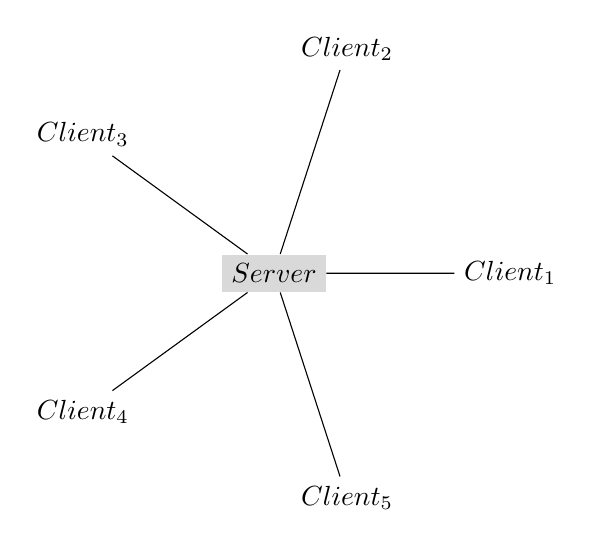
\begin{tikzpicture} [scale=1, transform shape]
%\tikzstyle{every node}=[draw,shape=circle];
\node [fill = gray!30] (v0) at (0:0) {$Server$};
\node (v1) at ( 0:3) {$Client_1$};
\node (v2) at ( 72:3) {$Client_2$};
\node (v3) at (2*72:3) {$Client_3$};
\node (v4) at (3*72:3) {$Client_4$};
\node (v5) at (4*72:3) {$Client_5$};
\draw (v0) -- (v1) % star
(v0) -- (v2)
(v0) -- (v3)
(v0) -- (v4)
(v0) -- (v5);
\end{tikzpicture}
\caption{客户\/服务器架构}
\label{CS}
\end{center}
\end{figure}






\subsubsection{P2P~架构}
% 好处与缺点

\begin{figure}[htbp]
\begin{center}
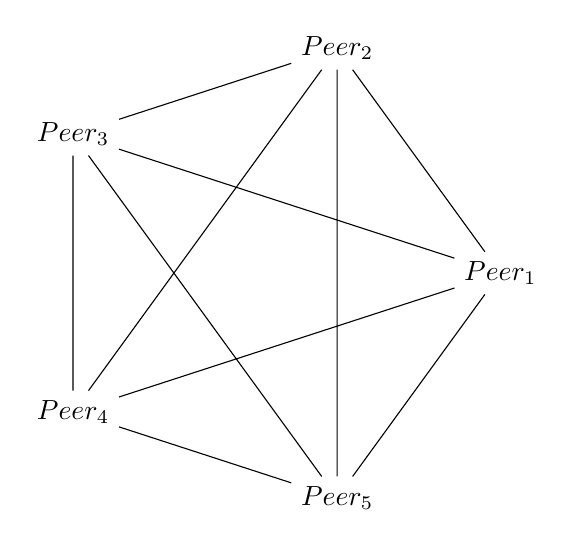
\begin{tikzpicture} [scale=1, transform shape]
%\tikzstyle{every node}=[draw,shape=circle];

\node (v1) at ( 0:3) {$Peer_1$};
\node (v2) at ( 72:3) {$Peer_2$};
\node (v3) at (2*72:3) {$Peer_3$};
\node (v4) at (3*72:3) {$Peer_4$};
\node (v5) at (4*72:3) {$Peer_5$};
\draw (v1) -- (v2) % fully connected
(v1) -- (v3)
(v1) -- (v4)
(v1) -- (v5)
(v2) -- (v3)
(v2) -- (v4)
(v2) -- (v5)
(v3) -- (v4)
(v3) -- (v5)
(v4) -- (v5);
\end{tikzpicture}
\caption{对等体架构}
\label{P2P}
\end{center}
\end{figure}


\subsubsection{分布式架构}
% 好处与缺点

\begin{figure}[htbp]
\begin{center}
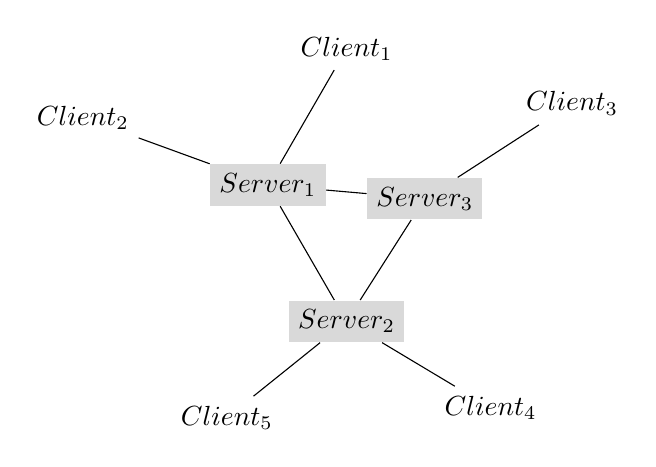
\begin{tikzpicture} [scale=1, transform shape]
%\tikzstyle{every node}=[draw];
\node [fill = gray!30] (s1) at (0:0) {$Server_1$};
\node [fill = gray!30] (s2) at (300:2) {$Server_2$};
\node [fill = gray!30] (s3) at (355:2) {$Server_3$};
\node (c1) at (60:2) {$Client_1$};
\node (c2) at (160:2.5) {$Client_2$};
\node (c3) at (15:4) {$Client_3$};
\node (c4) at (315:4) {$Client_4$};
\node (c5) at (260:3) {$Client_5$};

\draw (s1) -- (s2) -- (s3) -- (s1);
\draw (c1) -- (s1) -- (c2)
(c4) -- (s2) -- (c5)
(c3) -- (s3);

\end{tikzpicture}
\caption{分布式}
\label{distributed}
\end{center}
\end{figure}


%-------------------------------------------------%
\subsection{八项服务}
% 网络结构需要为游戏提供的八项服务(400字)
% 见意大利论文
\label{service}

一个完整的游戏架构应该提供以下八项服务:\cite{openping, dsl}

\begin{description}
\item[状态维护(State Maintenance)]
GSS~维护游戏状态。这个游戏状态包括虚拟世界和这个世界中所有角色的状态。

\item[一致性维持(Consistency Maintenance)]
由于不同的用户拥有不同的延时,因此他们各自看到的虚拟世界可能存在时间上的冲突和差异,因此需要提供一致性维持服务来减小甚至消除此种差异。

\item[群组管理(Group Management)]
对用户分组以及事件过滤服务也很有用,因为并非所有用户都希望得到一样的信息,这与游戏本身的语义和玩家的运算能力都有关。

\item[事件通知(Event Delivery)]
所有玩家都拥有平等的被通知权。不应该因技术原因使玩家收到通知的时间和质量存在差异。

\item[账号与认证(Accounting, Authorization)]
有时在游戏开始之初用户可以选择环境和设定参数。游戏可以通过账号来认证用户。

\item[作弊控制(Cheating Control)]
玩家的动作必须经检验才可以向其他玩家通知。一些有趣的防止作弊的方法如~\cite{cheat1, cheat2, cheat3, cheat4}。

\item[玩家间通信(Player Communication)]
玩家间实时的文字、音频、视频通信可以增强用户体验。

\item[多媒体资料传播(Multimedia Resource Distribution)]
传统观点中多媒体资料的传播仅仅局限于游戏开始之前的“离线”下载阶段。~\cite{traditional}~而新兴的观点则认为多媒体资料的下载将贯穿整个游戏过程,并增强用户间互动,提升游戏的可玩性。~\cite{modern1, modern2, modern3}
\end{description}
%-------------------------------------------------%

\subsection{一堆概念}
\label{def}
% 400字

%============================%

\section{传统~IP~网络中的经典同步机制}
\label{traditional}

\subsection{同步算法}
% 600字

\subsection{保守同步算法}

\subsection{优化同步算法}


%============================%

\section{新兴数据命名网络中的同步机制}
\label{innovative}
%(100字)

\subsection{CCN~中的~SYNC~协议}
% 800字

\subsection{用户自定义协议}
% 200字

\subsection{其它新型网络中的同步}
% 200字

\bibliography{data/zjubib}